\begin{refsection}
\renewcommand{\thefigure}{\arabic{figure}}

\chapterTwoLines
{Farinha e carne no sertão. Fome e caristia no litoral}
{aspectos do mercado interno no Rio Grande do Norte (séc. XVIII a XIX)}
\label{chap:farinha}

\articleAuthor
{Thiago Alves Dias}
{Doutor pelo Programa de Pós-Graduação em História Econômica da Universidade de São Paulo (PPGHE/USP), professor de História Moderna na UPE e pesquisador no grupo de pesquisa do CNPq ``Laboratório de Experimentação em História Social'' da UFRN. ID Lattes: 4789.9607.6279.7571. ORCID: 0000-0003-4308-418X. E-mail: thiago.dias@upe.br.}

\begin{galoResumo}
    \marginpar{
        \begin{flushleft}
        \tiny \sffamily
        Como referenciar?\\\fullcite{SelfDias2021}\mybibexclude{SelfDias2021}, p. \pageref{chap:farinha}--\pageref{chap:farinhaend}, \journalPubDate{}
        \end{flushleft}
    }
    Partindo da análise de dois gêneros básicos da alimentação colonial que foram objetos de regulação direta das instituições administrativas coloniais, a farinha de mandioca e a carne bovina, o presente artigo visa contribuir com a escassa discussão historiográfica norte-rio-grandense sobre o mercado interno e as dinâmicas mercantis coloniais durante o século XVIII e primeira metade do XIX, notadamente, da cidade do Natal. Com base nos registros da Câmara de Natal, cartas de sesmarias e outras fontes documentais, bem como amparado nas proposituras teóricas do historiador econômico Istvan Hont, concluímos que o comércio interno no Rio Grande do Norte, em geral, e na cidade de Natal, em particular, ganhou conjunturas de estabilidade e superação de problemas de abastecimento a partir da conquista colonial dos sertões e das prerrogativas institucionais de controle auferidas pela Câmara de Natal.
\end{galoResumo}

\galoPalavrasChave{Câmara de Natal. Rio Grande do Norte. Mercado interno.}

\begin{otherlanguage}{spanish}

    \fakeChapterTwoLines
    {Harina y carne en el sertão. Hambre y carestía en la costa}
    {aspectos del mercado interno en Río Grande del Norte (siglos XVIII al XIX)}
    
    \begin{galoResumo}[Resumen]
        Desde el análisis de los tipos básicos de alimentos coloniales que fueron objeto de regulación directa por parte de las instituciones administrativas coloniales, la harina de mandioca y la carne vacuna, este artículo tiene como objetivo contribuir a la escasa discusión historiográfica en el mercado interno de Río Grande del Norte y la dinámica mercantil colonial durante el siglo XVIII y la primera mitad del XIX, especialmente en la ciudad de Natal. Basándose en los registros de la Cámara de Natal, cartas de sesmarias y otras fuentes documentales, así como amparado en los planteamientos teóricos del historiador económico Istvan Hont, concluimos que el comercio interno en Río Grande del Norte, en general, y en la ciudad de Natal, en particular, ganó estabilidad y superó problemas de abastecimiento como resultado de la conquista colonial del interior y de las prerrogativas institucionales de control obtenidas por la Cámara de Natal.
    \end{galoResumo}
    
    \galoPalavrasChave[Palabras clave]{Cámara de Natal. Río Grande del Norte. Mercado interno.}
\end{otherlanguage}

\section{Introdução}

No mês de julho de 1711, a Câmara de Natal registrou em seus livros a falência de João do Rosário, o contratador das carnes daquele ano. Resolveram, portanto, notificar o fiador do contrato, o tenente-coronel e vereador Manoel Rodrigues Coelho, exigindo que o mesmo apresentasse uma solução para o caso. Naquela altura, Manoel Rodrigues Coelho já estava de volta a Natal, já que o mesmo estava nas trincheiras do Assú combatendo com os indígenas do sertão, sendo inclusive eleito no ano de 1712 a função de Juiz Ordinário da Câmara de Natal. Ocorre que durante o mês de junho daquele ano de 1711, mês festivo em torno do fim da colheita do milho e apropriado pelo calendário cristão em memória dos santos Antônio, João e Pedro; a cidade sofreu um verdadeiro desabastecimento de carne bovina\footnote{Instituto Histórico e Geográfico do Rio Grande do Norte [IHGRN] --- Livros de Termos de Vereação da Câmara de Natal [LTVCN], livro 1709--1721. Câmara de Natal. Termo de Vereação de 02 de julho de 1711, fl. 43v. Manuscrito.}.

No mês de maio de 1713, ou seja, em meio ao problema do abastecimento da carne bovina, a Câmara de Natal decidiu, acatando a queixa da população, instituir uma multa para os agricultores que fabricavam farinha de mandioca e não traziam para a venda pública na cidade do Natal\footnote{IHGRN --- LTVCN, livro 1709--1721. Câmara de Natal. Termo de Vereação de 23 de maio de 1713, fl. 77v-78. Manuscrito.}. Muito embora não houvesse impostos diretos da Câmara sobre a comercialização da farinha de mandioca, o que poderia encarecer o produto, como era o caso da carne bovina, a oferta do ``ordinário pão da terra'', como referiu-se Francisco de Brito Freire em 1630 \cite[p.~187]{Freire1675nova} e reiterado por Caio Prado Jr. em suas relevantes proposituras sobre a agricultura de subsistência no Brasil colonial \cite[p.~165]{PradoJr1997}, também sofria com as guerras no sertão. O abastecimento das tropas do Açu impedia que a produção de farinha do sertão viesse para o litoral. Além disso, parte considerável da farinha produzida no litoral seguia o lucrativo comércio com a capitania de Pernambuco, problema essa que teve continuidade durante todo o século.

Esse quadro de guerras coloniais contra os indígenas e a oferta de mercados mais vantajosos fora da Capitania do Rio Grande do Norte, provocou sucessivas ondas de desabastecimento na cidade de Natal durante o século XVIII: nem carne, nem farinha.

O presente artigo visa contribuir com a escassa discussão historiográfica norte-rio-grandense sobre o mercado interno e às dinâmicas mercantis coloniais durante os séculos XVIII e XIX, notadamente, da cidade do Natal. A problemática aqui discutida limita-se entre o fim das Guerras de Conquista do Sertão, a chamada ``Guerra dos Bárbaros'' (c. 1720), até, aproximadamente, a segunda metade do século XIX, quando a cotonicultura muda, drasticamente, os padrões de consumo e de circulação de produtos do comércio interno no Rio Grande do Norte.  

No tocante a historiografia, diferentes esforços de pesquisas em história econômica e social do Brasil, notadamente, a partir da década de 1970, tem se debruçado sobre as formas de organização e funcionamento dos circuitos mercantis internos no período colonial \cites{Linhares1979historia}{Lapa1980modos}. Passado mais de meio século, a crescente preocupação das humanidades com problemáticas permanentes, tais como: acesso à terra, desiguais relações de trabalho e ausência de políticas públicas de financiamento e intervenção estatal em áreas produtivas estratégicas, por exemplo, continuam conduzindo a comunidade acadêmica a investigar o nosso passado agrário. Essas pesquisas têm o mérito de buscar evidenciar, entre outras questões, as práticas comerciais endógenas e aspectos da economia de subsistência na América portuguesa, passando pela formação e consolidação de mercados internos. Esse esforço contínuo de produção de conhecimento visa nos auxiliar, enquanto sociedade, na definição de caminhos e estratégias para superação de parte desses nossos problemas históricos. 

Esse artigo partiu da análise de dois gêneros básicos da alimentação colonial que foram objetos de regulação direta das instituições administrativas coloniais: a carne bovina e a farinha de mandioca. A escolha deve-se ao fato de que inicialmente esses gêneros foram largamente produzidos no litoral atendendo as demandas populacionais proporcionais ao primeiro século da colonização. Com o adensamento populacional litorâneo, a consolidação da conquista dos sertões na primeira metade do século XVIII, foi uma alternativa para ocupação da terra e formação dos planteis, lavouras e pastos do sertão servindo de retaguarda as necessidades de abastecimento alimentício litorâneo. Apesar das insuficientes pesquisas realizadas no campo da alimentação e produção de alimentos na Capitania do Rio Grande do Norte, tudo nos leva a crer que o arroz, o milho e o feijão eram, sem dúvidas, amplamente consumidos, no entanto, tinham um papel secundário na alimentação cotidiana diante do consumo da farinha de mandioca. De acordo com Câmara Cascudo \citeyear[p.~78]{Cascudo1980}, “a farinha foi o produto inicial e sempre há citações holandesas e portuguesas [\dots]. A Capitania era região de gado e mandioca”. 

O trabalho de pesquisa aqui empregado segue as proposituras teóricas defendidas pelo historiador britânico da economia e do pensando político, Istvan Hont \citeyear{hont2005jealousy}. Para esse historiador, os padrões de desenvolvimento político europeu durante o período moderno, consolidadas durante o século XVIII, mas em franca expansão desde o século XV, passaram a alinhar o comércio como função do Estado moderno, solidificando a interação ``comércio e política'' e intervindo, inclusive, nas questões de mercado interno, economia doméstica e segurança alimentar das populações. As funções comerciais das instituições modernas que cuidavam da presença do rei e do aparato português no Brasil durante o período colonial não deixaram de ser afetadas por essas transformações e foi justamente nesse longo processo que podemos analisar um dos cruciais fatores que permitiram a formação das nações e do ideal do nacionalismo econômico tão preponderante no âmbito dos Estados nacionais no século XIX, inclusive no Brasil: a interação ``comércio e política''. 

Nesse sentido e buscando emular as questões teóricas à realidade política colonial e imperial do Rio Grande do Norte entre os séculos XVIII e XIX, a hipótese desenvolvida nesse artigo é que o comércio interno no Rio Grande do Norte, em geral, e na cidade de Natal, em particular, ganhou conjunturas de estabilidade e superação de problemas de abastecimento a partir da conquista colonial dos sertões e das prerrogativas institucionais de controle auferidas pela Câmara de Natal. Assim sendo, a conquista colonial dos sertões permitiu, por um lado, a ampliação das fazendas pecuaristas e das lavouras de mandioca nos sertões e, por outro lado, a Câmara de Natal passou a legislar e ser mais operante em proteção ao mercado interno e de subsistência, trazendo essa matéria para o centro das questões jurisdicionais  e da organização do estado burocrático local. 

Quanto as questões metodológicas, Maria Yedda Linhares \citeyear{Linhares1979historia}, já havia assinalado a urgência na pesquisa e aprofundamento da temática sobre o mercado interno, ressaltando a importância do desenvolvimento de estudos sobre a pecuária e a cultura de alimentos no Brasil, encarando-os em suas características internas e externas, assim como também se fazia necessário o estudo das interrelações territoriais. A pesquisadora também apontou um caminho metodológico quando afirmou ser indispensável retomar velhas fontes cartoriais e de natureza municipal, utilizar novas fontes, reavaliar outras já conhecidas e revalorizar velhos textos, de forma sistemática e organizada.  

Seguindo essas premissas, além da reavaliação de um antigo trabalho produzido sobre esse tema \cite{Dias2007carne}, utilizamos enquanto fontes documentais: registros das vereações da Câmara de Natal sob a guarda do Instituto Histórico e Geográfico do Rio Grande do Norte (IHGRN); cartas de sesmarias que explicitam as intenções de uso da terra dos solicitantes disponíveis na Plataforma Sesmarias do Império Luso-brasileiro (SILB); registros das ações dos Presidentes de Província do século XIX disponíveis no site do \textit{Center for Research Libraries}; correspondência entre autoridades do Rio Grande do Norte e administradores lusos através da documentação do Arquivo Histórico Ultramarino (AHU) do fundo Conselho Ultramarino e disponível no site da Biblioteca Nacional do Rio de Janeiro (BNRJ) e, por fim, documentos diversos publicados em periódicos como, por exemplo, “Memória sobre a extrema fome\dots” do padre Joaquim José Pereira de 1793 sobre a produção de alimentos no sertão do Rio Grande do Norte e publicado na Revista do Instituto Histórico e Geográfico Brasileiro (IHGB).

\section{A raiz indígena e o comércio da farinha de pau}

No final do século XVIII, o padre Joaquim José Pereira produziu importantes relatos e memórias  sobre os longos anos em que viveu no sertão da Ribeira do Apodi, na Capitania do Rio Grande do Norte, indo viver em São Luís no Maranhão em 1792. Até aquele ano, exerceu a função de vigário dos índios na Vila de Portalegre, “onde era a minha residência no emprego de Sua Majestade”. Na “Memória sobre a extrema fome e triste situação em que se achava o sertão da Ribeira do Apody da Capitania do Rio Grande do Norte\dots”, o padre registrou suas afetividades e denúncias sobre uma grande seca que assolou aquelas paragens no ano de 1792 em uma das memórias dirigidas ao Secretário de Estado dos Negócios da Marinha e Domínios Ultramarinos em Portugal, D. Rodrigo de Souza Coutinho, o futuro Conde de Linhares, enviada para Portugal em 1798 e publicada pela primeira vez na Revista do IHGB na edição de 1857 \cite{Pereira1973memoria}. 

O lamurioso relato do padre sobre a seca e a fome no sertão foi acompanhado de relevantes reflexões sobre a vida no sertão, a questão do acesso à água, a cadência das chuvas, a importância de se estocar alimentos, além de sofisticadas análises sobre o papel da agricultura e da terra na constituição dos Estados modernos. Parecendo ter saído de textos de François Quesnay sobre a questão do plantio e dos frutos da terra como aqueles que “enriquece os Estados e as monarquias mais do que todos os outros”, Joaquim José Pereira nos deixou um mapa. Esse curioso documento é uma tabela apensa à memória indicando, entre outras informações quantitativas, o número de habitantes daquelas paragens em 1792, a quantidade de suas plantações de mandiocas, o número dos lavradores empregados, a quantidade de farinha que consumiam e o excedendo que podiam estocar. 

De acordo com as informações constante, viviam na Ribeira do Apodi no ano de 1792, pouco menos de 9 mil pessoas, sendo que 5\% dessa população era constituída de lavradores de mandioca. Reunindo as informações das três freguesias que compunha aquela ribeira, ou seja, as margens do Apodi, a povoação de Pau dos Ferros e a Vila de Portalegre, plantou-se naquele ano 1.888.000 covas de mandioca, produzindo nada menos que 56.640 alqueires de farinha. De acordo com as estimativas do padre, cada individuo consumia um prato de farinha por dia e como um alqueire de farinha corresponde a 60 pratos, significa dizer que anualmente um individuo consumia 6 alqueires de farinha. As estimativas do padre nos surpreendem quando é constato que a produção de farinha de mandioca, em um ano de extrema fome e copiosa seca, apresenta um saldo positivo em mais de 4 mil alqueires de farinha. Significa dizer, portanto, que há produção de farinha para toda a população da Ribeira e um excedente pequeno, no entanto, possível de alimentar toda a população em mais um mês de seca, sem alterar os padrões de consumo mínimo de farinha de mandioca. É possível imaginar a quantidade de farinha produzida em tempos de chuvas regulares.  

Uma das perguntas possíveis e que vale a pena ser feita é: em que momento e a partir de que incentivos, as terras do sertão da Capitania do Rio Grande do Norte passaram a ser lavradas com mandioca e comportar engenhos de produzir farinha, tornando tal víveres um alimento básico e em níveis de produção positiva para a população local? Buscaremos apontar algumas respostas. 

Nativa da América do Sul e de conhecimento e usufruto originalmente indígena, a mandioca, palavra Tupi que significa ``casa de Mani'' ou ``raiz de Mani'', por causa de uma lenda indígena com variadas versões e investigada por Altino Brasil \citeyear{Brasil1987amazonia} através de entrevistas com caboclos e indígenas do Amazonas, é planta rica em calorias e de cultivo menos penoso comparado à produção açucareira ou aos cuidados que requeriam outros tipos de lavoura. Planta de fácil adaptação e resistente a seca, aproveita-se tanto as folhas, como sua suculenta raiz. Existem dois tipos de mandioca: a brava e a mansa. A mandioca brava é aquela que origina a farinha de mandioca, o ``pão do Brasil'', como afirmou o viajante inglês Henry Koster em 1810 \citeyear[p.~113]{Koster1942viagens} e precisa de dispendiosos preparos para tirar seu veneno e acidez e, só assim, produzir farinha, goma e outros subprodutos. Já a mandioca mansa é a macaxeira ou aipim e pode ser tirada da terra e logo preparada para o consumo. 

Se, por um lado, a iconografia produzida a partir do século XVII relaciona a planta e a raiz da mandioca ao mundo indígena, como podemos constatar nas pinturas de Albert Eckhout e analisadas pela pesquisadora Mariza de Carvalho Soares \citeyear{Soares2009engenho}, por outro lado, o trabalho nos engenhos ou casas de farinha, ou seja, a manipulação e o trabalho em torno da transformação da mandioca em farinha estão relacionados ao mundo africano. Essa forma e ordem de representações, ou seja, aos indígenas coube o conhecimento da planta e aos africanos coube o trabalho nos engenhos e casas de farinha, como pode ser constado nos exemplos apresentados no anexo iconográfico deste artigo, criou uma falsa ideia sobre o consumo alimentar.  

O alimento indígena não foi incorporado à alimentação colonial, logo em suas bases formativas, por um puro desejo das levas de europeus que chegavam nas américas. A ``farinha de pau'' foi uma solução alimentar encontrada pela Coroa e seus legisladores para assegurar o processo colonizador.  

É bem verdade que os rendimentos do açúcar de Pernambuco permitiram o pagamento das tropas e dos custos da guerra contra os Potiguaras no século XVI e a efetiva conquista do Rio Grande. Mas é igualmente verdade que o envio de 50 alqueires de farinha de mandioca, às custas da população litorânea e a mando da Câmara de Natal para manter as tropas nas Guerras de Conquista do Sertão no Assú no final do século XVII, foi importante para o sucesso da empreitada colonial nos sertões\footnote{IHGRN --- LTVCN, livro 1674--1698. Câmara de Natal. Termo de Vereação de 02 de ago. de 1687, fl. 74v. Manuscrito.}. Uma década mais tarde, com a continuidade das guerras contra os indígenas do sertão, “todos os moradores de mais posição” da Cidade do Natal, decidiram manter às suas expensas, um presídio em Assú com “farinhas para o sustento dos que nelas assistissem” por 6 meses, enquanto uma das soluções apresentadas pelo Capitão-mor ao rei D. Pedro II “para segurança e aumento das povoações”\footnote{Arquivo Histórico Ultramarinho [AHU] --- Conselho Ultramarino, RN, cx. 1, doc. 42. Carta do Capitão-mor do Rio Grande, Bernardo Vieira de Melo, ao rei D. Pedro II sobre as decisões dos oficiais da Câmara e moradores de Natal de se fazer um presídio no sertão do Açu, que seria sustentado por seis meses pelas farinhas dadas pelos moradores. Natal, 15 de abril de 1697. Manuscrito.}.

Como assinalou Bert Barickman \citeyear{Barickman2003acucar}, mais do que a preocupação com o sustento dos escravos, a insistente reedição de alvarás e provisões régias, ainda na primeira metade do século XVII, que obrigavam os senhores de engenho e lavradores de cana a plantar um número mínimo de covas de mandiocas, era para assegurar os estoques abundantes de farinha para os mercados locais e as populações coloniais como um todo. 

Nenhuma das cartas de sesmarias da Capitania do Rio Grande do Norte, ou seja, os títulos de concessão de terras, citam, como justificativa para a petição, o plantio de mandioca. Mesmo assim, alguns registros mencionam terras para lavoura ou plantio, como foi o caso da viúva Paula Pereira de Abreu, que requereu uma sesmaria na cidade de Natal concedida em 1735 alegando “não ter terras para o plantio de lavouras”\footnote{Plataforma SILB --- RN 1149. Carta de Sesmaria de Paula Pereira de Abreu. Concessão em 01 de jan. 1735. Disponível em http://www.silb.cchla.ufrn.br.}. A ausência de registro de solicitações de terras com justificativas em torno da mandioca não implica dizer que não houve lavradoras ou lavradores de mandioca, ou engenhos e casas de farinha na Capitania.  

Para além da subsistência alimentar das famílias que produziam sua própria farinha, as demandas em torno da comercialização interna, sobretudo, durante o século XVIII, deu-se muito mais em função das normativas camarárias que passaram a intervir diretamente na produção agrícola para fomento e proteção do comércio interno de farinha de mandioca, do que as iniciativas particulares dos lavradores ou comerciantes de farinha que acabavam exportando sua produção para o comércio intracapitanias, notadamente, para Pernambuco. 

Os primeiros registros disponíveis sobre o ordenamento institucional por parte da Câmara de Natal acerca do plantio de mandioca datam da segunda metade do século XVII e passam a ser constantes. As ordens camarárias para o plantio mínimo de covas de mandioca, controle na saída desse gênero para fora da Capitania e as punições para quem descumprisse essas diretrizes, foram temas recorrentes por parte da Câmara de Natal durante todo o período colonial, sobretudo, em períodos de estiagem. As Posturas anuais, editais e a reedição constante de punições para os que descumprisse os valores sobre preços praticados ou que vendessem para fora da Capitania também foram discutidos na Câmara. No ano de 1734, por exemplo, a Câmara de Natal resolveu convocar os lavradores de mandioca em reunião para avaliar a capacidade de produção de suas roças, objetivando forçar os lavradores a manter um fornecimento de farinha para o mercado interno com alguma regularidade\footnote{IHGRN --- LTVCN, livro 1721--1735. Câmara de Natal. Termo de Vereação de 03 de março de 1734, fl. 154v--155v. Manuscrito.}. Como apontou Barickman para a realidade da cidade de Salvador durante o período colonial, “a repetição dessas leis é por si mesma sugestivas; se tivessem sido obedecidas, não teria sido necessário reeditá-las a cada ameaça de escassez” \cite[p.~105]{Barickman2003acucar}. 

Três mecanismos de fomento à produção de farinha e controle comercial desse produto foram utilizados de forma mais constante pela Câmara para garantir o abastecimento regular interno: vigilância nas roças, vigilância no comércio e solicitações de envio de farinha dos sertões para o litoral. Mas não foram os únicos.  

Muito embora, após o fim das Guerras de Conquista do Sertão e a efetiva transformação da paisagem nativa em espaços coloniais, a oferta da farinha de mandioca tenha sido alterada pela produção sertaneja, o problema do mercado interno não deixou de ser pauta na Câmara de Natal, muito em função do interesse dos lavradores em venderem a farinha para fora da Capitania, como já foi apontado. A lista de ações é extensa: regular o preço máximo do alqueire a ser vendido ao povo; promulgação de multas e penalidades para os descumpridores das normativas; pagamentos de aforamento das terras da Câmara foram cobrados em farinha; vadios foram coagidos para trabalhar nos roçados; roças foram averiguadas; roceiros foram notificados para declararem, sob juramento, quanto plantavam e quanto de farinha produziam; farinha foi apreendida nas casas, roças e porto etc.  

Dentre essas ações insistentes e repetitivas da Câmara de Natal, uma ordem expedida em 1778 se sobressai: a assinatura de um compromisso por parte de alguns importantes senhores de terras e comerciantes da Capitania em enviar 20 alqueires de farinha, cada um\footnote{IHGRN --- LTVCN, livro 1766--1781. Câmara de Natal. Termo de Vereação de 02 de março de 1778, fls. 240--240v. Manuscrito.}. Entre os signatários que assinaram o compromisso com a Câmara de trazer a farinha de mandioca para a venda em Natal estavam: os capitães Manoel Álvarez de Morais Navarro, descente da família francesa Navarro com posses de terra e negócios na capitania desde a primeira metade do século XVII \cite{Dias2016gentes}; Antônio da Silva de Carvalho e o Manuel de Abreu Soares, todos detentores de terras no litoral quanto no sertão, o que provavelmente indica que possuíam roçados e até engenho/casas de farinha. Já o alferes João Pedro de Sá Bezerra e os sargentos-mores Prudente de Sá Bezerra, Antônio Rodrigues Santiago e José Rodrigues da Rocha, além de Francisco Gomes, possuíam terras no litoral, mas sem menção a posses no sertão, o que não impedia que mantivessem roçados e lavradores de mandioca nas suas terras ou fossem comerciantes ou mesmo os dois. Como era de se esperar, nem todos cumpriram o acordado, no entanto, esse expediente de convocar pessoas nominalmente para fornecerem farinha foi se repetindo nas decisões da Câmara. 

Antônio da Silva de Carvalho, meses depois, foi notificado mais uma vez de seu compromisso assumido e Manoel Álvares de Morais Navarro, embora aparentemente tenha atendido a Câmara naquele momento, anos depois, em 1786, foi notificado para conduzir à Natal “toda a farinha em seu poder”, por constar que pretendia comercializar nas regiões salineiras, fora da jurisdição da Câmara, para ser exportada para Pernambuco, “em extremo prejuízo ao Povo, o que já teria acontecido para outros destinos”\footnote{IHGRN --- LTVCN, livro 1784--1803. Câmara de Natal. Termo de Vereação de 1786 (data ilegível), fl. 29. Manuscrito.}.  

Durante a segunda metade do século XVIII é possível constatar que foi mais recorrente a vigilância em torno da farinha que seguia para fora da Capitania, fosse através dos caminhos terrestres, fosse através do movimento portuário nas áreas salineiras. A Câmara de Natal não só reeditou incansavelmente suas ordens e éditos sobre a farinha de mandioca, como passou a intervir em outras jurisdições ou envolver outros agentes e instituições administrativas nessa empreitada: “solicitaram do Governo da Capitania providenciar farinha de outras jurisdições que não fossem desta Câmara”, “solicitaram dos Capitães-mores da Capitania que impedissem o embarque de 200 alqueires de farinha para Pernambuco”\footnote{IHGRN --- LTVCN, livro 1784-1803. Câmara de Natal. Termos de Vereação de 1786 (data ilegível), fl. 27v-28. Manuscrito.} e até mesmo pedidos para aqueles que tivessem roças e morassem fora da Capitania, trouxessem farinha.

A farinha de mandioca, “presente tanto nas mesas dos ricos, como na dos pobres, e nas cuias e baldes  que os escravos usavam à falta de pratos, constituía a base da dieta comum” \cite[p.~96]{Barickman2003acucar} e foi largamente produzida nos sertões da Capitania do Rio Grande do Norte, como foi demonstrado na memória do pe. Joaquim José Pereira, como também em áreas adjacentes a Natal. Foi produto de grande relevância comercial ao ponto de ter provocado desabastecimento e inflação do preço, já que os alqueires de farinha de mandioca seguiam para mercados de exportação mais rentáveis.   

Ao final do século XVIII, a situação de segurança alimentar em Natal continuava fragilizada sob a pressão do mercado exportador, notadamente, do comércio realizado com a Capitania de Pernambuco. Em 1791, o Capitão-mor Caetano da Silva Sanches escreveu aos agentes metropolitanos em Lisboa suas diligências a frente da Capitania e afirmou que a venda de farinha em Natal, durante meses “se não vendia aqui uma quarta”, uma vez que a farinha era conduzida em embarcações para diversas partes” e a pouca que permanecia era vendida inflacionada, dada a grande procura\footnote{AHU --- Conselho Ultramarino, RN, cx. 8, doc. 483. Ofício do Capitão-mor do Rio Grande do Norte, Caetano da Silva Sanches, ao secretário de estado da Marinha e Ultramar em Lisboa, Martinho de Melo em Castro. Natal, 29 de abril de 1791. Manuscrito.}. O novo capitão-mor cuidou em buscar intervir, com a força da lei e de sua jurisdição, talvez sem saber que durante décadas à Câmara de Natal fez o mesmo e com pouco sucesso. 

Nesse sentido, coube as instituições ligadas ao aparato estatal, sobretudo, a Câmara de Natal, órgão a serviço do povo e dos interesses coloniais portugueses, buscar manter as condições de crescimento populacional e o desenvolvimento da cidade sede da Capitania, contingenciando os problemas de abastecimento alimentício internos recorrentes, adotando medidas que implicavam diretamente na relação ``política'' e ``comércio''. 

Durante a segunda metade do século XIX e no contexto do surto epidêmico do cólera-morbo que se estendeu entre 1855 a 1857 na província, mesmo mediante todos os esforços perpetrados pela Câmara de Natal séculos antes para tornar mais seguro a oferta de farinha no mercado interno, a fome foi recrudescida. A fala de um presidente de província acerca da possível atitude da população resumiu os ânimos vividos naqueles tempos de penúria e fome: “ou farinha ou revolução” \cite[p.~117]{Monteiro2007terra}. Naquela ocasião e mais uma vez, foi a interferência do estado que sanou a crise alimentar com envios de farinha de mandioca pelo Governo Imperial no Rio de Janeiro e uso dos recursos públicos para compra do mesmo nas províncias vizinhas de Pernambuco e Ceará.

\section{O boi europeu e o comércio da carne vacum}

É consenso entre os pesquisadores da alimentação que a mais expressiva revolução nos hábitos alimentares humanos foi vivenciada durante o período moderno e fruto da expansão colonial europeia, provocando um maior intercâmbio de produtos de diferentes continentes e alterando, indelevelmente, a dieta e o paladar de praticamente todos os povos do mundo. Esse foi o caso do consumo da carne de boi e de vaca na alimentação no Brasil desde o século XVI.

Tanto os registros escritos como as escavações arqueológicas confirmam que na antiguidade do continente europeu, a criação de bois era muito difundida no trabalho dos campos, especialmente na lavoura e, portanto, seu papel na alimentação era secundário. Essa relação se modifica durante a Idade Média, já que as escavações revelam a presença significativa de ossos de bois nos restos de cozinha, mesmo mantendo a prerrogativa de abater os animais idosos, já que os jovens puxavam os arados e as carroças \cite{Flandrin1998historia}. Embora a agricultura produza muito mais alimentos do que a criação de gado em uma mesma extensão de terra, foram os povos europeus modernos que mais valorizaram a alimentação carnívora e promoveram a ideia de criação sistemática e regular de caprinos, ovinhos e bovinos voltados, em grande medida, para o abate e alimentação, ligados ao ritmo de reprodução dos animais e sua aceleração quando pensado em conjunto no rebanho \cite{Carneiro2003comida}.

Embora as populações nativas americanas se alimentassem de carne de animais silvestres, as carnes de caça, sua dieta alimentar não era baseada no consumo exacerbado de alimentos cárneos. Mesmo após o contato e intercâmbio de sabores e experiências alimentares entre indígenas e europeus, os indígenas mantiveram a distinção entre os animais criados na companhia de coletivos humanos e os alimentos provenientes da caça \cite{Velden2019tratados}.

O gado doméstico europeu, descendente de espécies de bovinos silvestres que habitaram tanto a Ásia com a África, levou milhares de anos para sua domesticação, no entanto, desde as primeiras levas de gado bovino que Colombo transportou das Canárias para Hispaniola no final do século XV, este foi rapidamente naturalizado, representando mais um elemento triunfante da ``biota portátil'' que os europeus conduziram para as américas \cite{Crosby1993imperialismo}.

No caso da conquista colonial da Capitania do Rio Grande, notadamente, a partir da formação da cidade de Natal em 1598-99, o projeto colonial do gado foi a solução colonizadora encontrada, já que as terras não eram propícias para o açúcar. Terras boas para o gado de todas as sortes: vacum, cabrum, ovelhum, muares. Dos 1.268 registros de terras da Capitania do Rio Grande do Norte disponíveis na Plataforma SILB, 857 citam como justificativa de petição da terra o criatório bovino. Ou seja, quase 70\% de toda a terra da Capitania do Rio Grande do Norte foi solicitada para a pecuária. Uma pequena parcela desses registros se refere a terras para pescarias, chãos de terras nas áreas urbanas ou justificativas várias.

Já no século XVIII, o processo de ocupação colonial dos sertões, que não foi tranquilo e nem isento de disputas \cites{Araujo2007}{Alencar2017}, também foi consolidado pelo criatório bovino. Aos poucos, como explicou Muirakytan Macêdo \citeyear{Macedo2007rusticos}, o sertão da Capitania, “movidos pela abertura de fronteiras que possibilitaram a animação do mercado interno com a comercialização do gado”, deram início a um grande reordenamento demográfico, catastrófico, em grande medida, para os indígenas, mas rico de novos reordenamentos sociais. Esse quadro de ocupação colonial dos sertões pela pecuária, em grande medida, é confirmado também por meio da análise global das sesmarias nas Capitanias do Norte estudadas por Carmen Alveal \citeyear{Alveal2019}. No caso da Ribeira do Assú, esse custoso e violento processo de transformação de territórios nativos em espaços coloniais, criou uma dinâmica mercantil pujante, em que triunfaram as fazendas de criar gado, as olarias e as oficinas de charqueadas \cite{Silva2015}.

O gado, por sua vez, foi se alastrando nas paragens sertanejas e multiplicando-se em proporções cada vez maiores, durante todo o período colonial. Força motriz, leite, manteiga, queijo, carne, couro, gordura animal. Muitas foram as aplicabilidades do gado e sua utilização, tanto no cotidiano da subsistência (no âmbito da alimentação, vestuário e utensílios domésticos) como nos circuitos mercantis coloniais internos e de exportação.

A partir da análise de alguns registros iconográficos presentes no anexo desse artigo, podemos constatar que o motivo e seus variantes ``gado bovino'' foi representado em, pelo menos, três tópicos distintos: primeiro; força motriz que carrega o arado, puxa

a carroça e movimenta o engenho, notadamente, nos registros do século XVI e XVII e, portanto, uma relação com a noção de força e trabalho; segundo; registros de ferro com iniciais de nomes de indivíduos, famílias, fazendas ou localidades a serem afixados na pelo do gado, notadamente, nos registros dos séculos XVII a XIX e, portanto, uma relação com a noção de posse e jurisdição e, por fim, representações sobre alimentos, cozinha e comidas, notadamente, nos registros do século XIX em diante e, portanto, uma mudança de atitude sobre o preparo das carnes bovinas e seus derivados, muito em função da nova ordem imperial do Brasil e a circulação de livros de receitas a partir de impressos do Rio de Janeiro.

No tocante a relação entre alimentação e políticas municipais da Câmara de Natal para garantir a oferta de carne bovina para a população local, objeto principal de análise do artigo, as questões sobre a farinha de mandioca se repetem em relação a carne.

Os primeiros registros da Câmara de Natal da segunda metade do século XVII sobre a temática do abastecimento alimentar da carne versam sobre a regularização e aferição do preço máximo que deveria ser comercializado, indicando que o preço da carne bovina sofria inflação constante. Outro tema repetitivo foi a questão do abate de animais em casas particulares e sem licença da Câmara, já que prejudicava os rendimentos municipais e seu controle efetivo sobre o comércio local. No entanto, o objeto de maior preocupação dos camarários durante o século XVIII foi mesmo a falta de carne no mercado local da cidade.

A incisiva preocupação da Câmara sobre a falta de carne na cidade não impactava somente os níveis de confiança que a população poderia ou não ter sobre a gestão municipal. Impactava diretamente as contas da Câmara, já que era um dos poucos impostos de arrecadação municipal e que pagavam as próprias despesas da Câmara, tais como: o salário do escrivão e do porteiro, a compra de insumos como papel e tinta, a aquisição de velas e adornos para as celebrações que envolviam a Câmara ou mesmo a possibilidade de empenhar recursos em alguma obra pública de melhoria na cidade.

Havia um verdadeiro desinteresse dos comerciantes e fazendeiros em arrematarem o contrato municipal dos subsídios das carnes, ou seja, o contrato de cobrança de impostos devido à Câmara pela carne vendida no açougue público. Por um lado, essa era a forma dos próprios comerciantes e fazendeiros boicotarem a cobrança dos impostos, abatendo seus animais fora da área urbana da cidade. Por outro lado, esse desinteresse por parte dos possíveis indivíduos aptos a deterem o contrato demonstra a ausência de oferta regular de carne no mercado local, o que traria prejuízo aos possíveis contratantes, uma vez que o contrato era pago antecipado à Câmara por um valor arrematado e o arrematante ia retirar o capital investido e o lucro na cobrança diária da venda da carne. Na segunda metade do século XVIII, esse problema se agravou já que a criação do imposto régio sobre cada cabeça de boi abatida, o Subsídio Literário, aumentou a tributação sobre a carne bovina.

Se, na primeira metade do século XVIII, havia uma insegurança alimentar na cidade de Natal e a oferta de carne bovina era escassa, o fim das Guerras de Conquista do Sertão e a consolidação da ocupação colonial sertaneja voltada para a pecuária significou um alento.

Em 1783, a Câmara de Natal escreveu uma carta ao Juiz Ordinário do Julgado do Assú, José Caetano da Costa, explicando que motivações menores já seriam o bastante para a Câmara recorrer a outras jurisdições e se mover em vigilante cuidado, caso não fosse a grande falta de um dos principais alimentos que os habitantes de Natal experimentavam, “com grande e lastimosa frequência”. Muito embora a situação da fome e carestia alimentar estivesse implicada em decorrência da seca que a Capitania passava naqueles anos, a fala lamuriosa cita uma falta recorrente de carne bovina e não pontual.

A solução encontrada nessa ocasião foi cobrar da sociedade colonial sertaneja os envios de farinha que a sociedade colonial litorânea tinha desprendido anos antes para assegurar o genocídio das populações indígenas na ``Terra dos Tapuias''.

A Câmara de Natal remeteu ao Juiz do Assú um rol de 12 pessoas que deveriam conduzir cada um 16 rezes, duas vezes por mês, totalizando 32 cabeças de gado mensais durante seis meses, do sertão do Assú para Natal. Nesse sentido, entre os meses finais de 1783 e os iniciais de 1784, os fazendeiros da Ribeira do Assú deveriam conduzir 192 cabeças de gado cada um para a sede do governo da Capitania\footnote{IHGRN --- Livro de Registro de Cartas e Provisões da Câmara de Natal [LRCPCN], cx. 04, lv. 12. Câmara de Natal. Registro de uma carta que este Senado escreveu ao Juiz do Assú, José Caetano da Costa, em 16 de agosto de 1783 para efeito de mandar gado para o povo desta cidade. Natal, 16 de agosto de 1783. Manuscrito.}. Os 12 fazendeiros da Ribeira que aparecem no rol são: João da Costa Pinheiro, Sargento-Mor Francisco José Dantas, Capitão Francisco Dantas Cavalcante, Antonio Duarte, Tenente Constantino dos Santos Braga, Alferes Antonio Lourenço Pereira, José Pedro Tinoco, Capitão José Freire Carneiro, José Roiz, Capitão João Soares Salgueira, Tenente Cosme Damião e o Tenente Miguel da Rocha Marques.

Dentre esses fazendeiros dois nomes se destacam. Constantino dos Santos Braga detinha terras no Assú e em 1762 requereu a concessão de mais terras no sertão\footnote{Plataforma SILB — RN 0806. Carta de Sesmaria de Constantino dos Santos Braga. Disponível em http://www.silb.cchla.ufrn.br.}. Já José Pedro Tinoco requereu a Câmara de Natal, em 1787, um título de sesmaria de uma légua de terra que se iniciava em um poço d’água e seguia o curso do rio Assú, junto com sobras de terras que se encontravam devolutas próximas ao sítio de Angicos, atual cidade de Angicos, além de outras sobras de terras entre o riacho Juazeiro e o sítio das Flores, no rio Salgadinho, entre as confrontações do Riacho da Volta, ou seja, terras entre rios e águas, bastante propícias à pecuária\footnote{Plataforma SILB — RN 0884. Carta de Sesmaria de Jose Pedro Tinoco. Disponível em http://www.silb.cchla.ufrn.br.}.

Tal como foi solicitado que os fazendeiros da Ribeira do Assú levassem cabeças de gado de suas fazendas para Natal, dez agentes mercantis da Ribeira do Seridó também foram solicitados a trazer cabeças de gado em 1785. De acordo com uma outra carta, dessa vez enviada ao Coronel Caetano em 18 de junho de 1785, os camaristas afirmam que devido “à grande vexação em que se passa este povo está por falta de carne faz com que este Senado, como tendo obrigação, e procure remédio a este mal”, para tanto, foi remetido ao Regente dessa Ribeira “um rol em que vão nomeadas as pessoas que em cada mês vão mandar para esta cidade o determinado número de rezes e ainda que V. Mercê vai nomeado no mesmo rol”\footnote{IHGRN --- LRCPCN, cx. 4, lv. 12. Câmara de Natal. Registro de uma carta que este Senado mandou ao Coronel Caetano Dantas na Ribeira do Seridó. Natal, 18 de junho de 1785. Manuscrito.}.

Desse rol, consta o nome de dez senhores de fazendas que deveriam suprir com carne a cidade de Natal a partir de julho até dezembro de 1785, totalizando 175 cabeças de gado. Foram eles: o próprio Coronel Caetano Dantas, João Damasceno, Sargento-Mor regente Cipriano Lopes Galvão, Capitão Antonio da Silva, Cosme Soares, Felipe de Moura, Capitão Domingos Alves dos Santos, Manoel Gonçalvez de Mello, Manoel de Souza Forte e Vicente Fernandes.

A historiografia norte-rio-grandense, sobretudo, aquela produzida por memorialistas, cronistas e historiadores que residiam em vilas e cidades da Ribeira do Seridó, aponta Caetano Dantas e, posteriormente, seus descendentes, como homens e mulheres de grande influência e prestígio socioeconômico na região. Olavo de Medeiros Filho compilou uma série de documentos pertencentes a acervos do Rio Grande do Norte e da Paraíba que mostram a trajetória mercantil de Caetano Dantas. A caráter de exemplo, só na Ribeira do Seridó, entre os anos de 1742 a 1768, Caetano Dantas recebeu a confirmação de pelo menos sete sesmarias em lugares distintos ou ampliando as que já possuía, quase todas citando a criação de gado e lavouras. Ao problematizar a estratégia e evolução fundiária de Caetano Dantas Correa, Muirakytan Macêdo \citeyear[p.~81]{Macedo2007rusticos}, considera sua trajetória uma sístole, ou seja, “o processo de concentração fundiária por aquisições de sobras desaproveitadas e através da compra”.

Tendo passado a Tenente Coronel de Milícias em 1793, Caetano Dantas faleceu poucos anos depois. No seu inventário datado de 1798, ele deixou algumas fazendas de gado, casas e um montante equivalente a 5:673\$240 \cite[p.~120--121]{MedeirosFilho1983velhos}. Se tomarmos como parâmetro de comparação os totais do montante de produção da Capitania para o ano de 1811, os bens deixados por Caetano Dantas, em 1798, corresponderam a mais de 2\% de toda a riqueza da Capitania em mãos de um único agente mercantil \cite{Dias2007carne}.

As conexões entre as famílias dos fazendeiros podem ser constatadas através dos familiares de Caetano Dantas Corrêa e os sujeitos arrolados no rol. João Damasceno Pereira, que também foi convocado a remeter cabeças de gado para Natal, por exemplo, era irmão da esposa de Caetano Dantas. Já Cosme Soares Pereira, também convocado a remeter cabeças de gado, era irmão de João Damasceno Pereira e, portanto, também cunhado de Caetano Dantas. Já Cipriano Lopes Galvão, de acordo com Olavo de Medeiros e suas pesquisas da tradição oral, foi o primeiro Coronel do Regimento de Cavalaria da Ribeira do Seridó. Falecendo em 1813, deixou em seu inventário 23 escravos, 631 bovinos, 121 cavalos e 202 caprinos e ovinos. Dos dez títulos de terra deixados por Cipriano Lopes Galvão, oito eram de criar gados. Seu padrasto foi Antonio da Silva e Souza, também convocado pela Câmara de Natal para conduzir gado \cite{MedeirosFilho1983velhos}. O Sargento-Mor das Milícias, Felipe de Moura e Albuquerque deixou um farto inventário que, dentre outros bens, constava 1.066 bovinos, 85 cavalos, 42 caprinos e 24 escravos, um número maior que a média de escravos utilizados nas lides pecuaristas dos sertões da Capitania do Rio Grande do Norte \cite{MedeirosFilho1981velhas}.

A prática de recorrer ao gado do sertão para suprir as necessidades proteícas da população de Natal foram ficando cada vez mais expressivas e recorrentes.

A década de 1790 foi marcada por um grande período de estiagem na Capitania do Rio Grande, como foi discutido no início desse artigo sobre a produção de farinha de mandioca no sertão pela pena do padre Joaquim José Pereira. Como forma de garantir o abastecimento, a Câmara designou, por escolha do conselho, as pessoas que deveriam efetivar as responsabilidades dos contratos sem pagar diretamente à Câmara por isso. O sistema de ``administração pela Câmara'' escolhia entre os ``homens bons'', do termo da cidade, uma ``pessoa idônea e capaz'' que pudesse dar continuidade ao abastecimento da carne e da vigilância dos demais gêneros, passando a quinta parte de tudo que fosse arrecadado à Câmara.

Assim sendo, José Joaquim Ferreira Nobre foi o votado pela Câmara para permanecer atuando no contrato das carnes a partir de 1794. As motivações pela escolha do postulante foram apresentadas: “negociante de gado que vai comprar pelo sertão e por este ter muita carne”\footnote{IHGRN --- LTVCN, livro 1784--1803. Câmara de Natal. Termos de Vereação de 14 de junho de 1786, fl. 25. Manuscrito.}. Contrariando uma Provisão Régia, a Câmara de Natal estava disposta a não cobrar o imposto devido sobre cada arroba de gado, o Subsídio Literário, no intuito de fazer com que um comerciante, já participante dos ofícios régios, mesmo que temporário, trouxesse sua vasta produção de carne sertaneja para ser comercializada em Natal.

Muito embora durante todo o século XVIII os oficiais camarários tenham buscado soluções para o problema do abastecimento da carne bovina na cidade, o desinteresse dos negociantes em arrematar o contrato era sintomático. Por um lado, peixes, aves e animais menores podiam suprir a necessidade proteica da população, já que a pouca oferta da carne bovina era oriunda das fazendas sertanejas, o que inflacionava o preço final que chegava ao consumidor no litoral. Por outro lado, o corte e comércio da carne era realizado, até onde fosse possível, longe da interferência da Câmara que cobrava seus pesados tributos, encarecendo o produto. De uma forma ou de outra, durante século XVIII, a Câmara de Natal buscou diferentes estratégias de regularização da oferta de carne bovina a ser realizado dentro do açougue público: abriram mão dos autos de arrematação, bem como parte das pensões e impostos devidos; proibiram porcos e cabras na cidade alegando saúde pública e até instituíram “olheiros” para vigiar aqueles que estavam abatendo reses e cortando carne sem licença nas imediações. No entanto, foi o gado proveniente do sertão, fruto do processo colonizador baseado na pecuária após as Guerras de Conquista no Sertão, que trouxeram algum alento para a oferta de carne bovina em Natal.

Durante a primeira metade do século XIX a economia pecuarista do sertão continuou provendo as necessidades do litoral. Antônio Bernardo de Passos, Presidente de Província do Rio Grande do Norte, afirmou em 1854 que das fontes dos rendimentos da Província, o dízimo do gado era o mais importante até aquele ano. Essa constatação de Antônio Passos é fundamentada pelos seguintes dados: o dízimo do gado representou, em média, 47\% de todas as rendas provinciais do Rio Grande do Norte entre 1851 a 1854 \cite[p.~30]{Passos1854}. Como declarou também Figueiredo Jr., outro Presidente de Província, “até o ano de 1847, a criação de gado era a indústria quase exclusiva a que se aplicavam os habitantes da província” \citeyear[p.~37]{FigueiredoJr1861}. Depois da década de 1850, o algodão passou a ter maior expressividade no comércio e nas contas públicas. Muito embora o algodão não se coma, mas se veste, a prosperidade econômica da cotonicultura garantiu novos padrões de desenvolvimento e consumo as populações tanto no litoral, quanto no sertão. 

\section{Considerações finais}

A formação e consolidação do Estado moderno não foi produto somente da Europa, mas também passou pela experiência e prática das instituições coloniais na América entre os séculos XVI a XVIII. O ‘ciúme do comércio’, ou seja, a aplicação da razão do Estado nas questões comerciais e nas necessidades sociais ligadas ao comércio, como entende Istvan Hont \citeyear{hont2005jealousy}, também foi vivenciada na prática colonizadora ultramarina. A Câmara de Natal interveio diretamente nas questões comerciais e até produtivas para garantir o abastecimento e a oferta, com preços regulados, de farinha de mandioca e de carne bovina à crescente população que ia se instalando na cidade sede do governo da Capitania.

As tarefas e incumbências da Câmara não se restringiram a cobrança dos impostos devidos e da regularização das práticas e dos espaços comerciais, como fiscalizar lojas, aferir pesos e medidas ou manter o funcionamento de açougues e ordenamento de feiras livres. A Câmara buscou garantir a segurança alimentar das populações intervindo diretamente nas práticas comerciais e inclusive interferindo em outras jurisdições e espacialidades como o sertão, trazendo descontentamentos e afetando as lógicas de livre mercado que iam se instaurando, paulatinamente, no cotidiano das práticas mercantis e nas consciências dos que agentes mercantis.

Nesse sentido, o comércio interno no Rio Grande do Norte, em geral, e na cidade de Natal, em particular, ganhou conjunturas de estabilidade e superação de problemas de abastecimento a partir da conquista colonial dos sertões na segunda metade do século XVIII e das prerrogativas institucionais de controle auferidas pela Câmara de Natal durante todo o período colonial. A conquista colonial dos sertões permitiu, por um lado, a ampliação das fazendas pecuaristas e das lavouras de mandioca nos sertões e, por outro lado, a Câmara de Natal passou a legislar e ser mais operante em proteção ao mercado interno e de subsistência, trazendo essa matéria para o centro das questões jurisdicionais e da organização do estado burocrático local. 

\printbibliography[heading=subbibliography,notcategory=fullcited]

\hfill Recebido em 30 abr. 2021.

\hfill Aprovado em 14 maio 2021.

\label{chap:farinhaend}

\cleardoublepage

\begin{vplace}
    \section*{Anexo iconográfico: mandioca e carne bovina entre os séculos XVII e XIX}
    \addcontentsline{toc}{section}{Anexo iconográfico: \textit{mandioca e carne bovina entre os séc. XVII e XIX}}
\end{vplace}

\cleardoublepage

\begin{center}
    
\begin{tikzpicture}
    \node[inner sep=0pt] (tupinamba) at (0, 0)
        {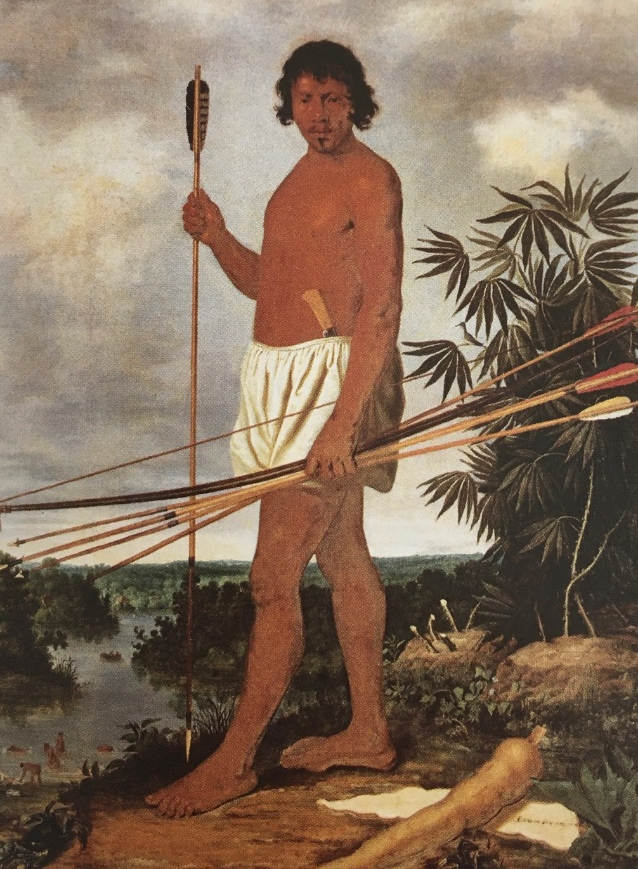
\includegraphics[width=50mm]{arcticles/02-farinha-e-carne-no-s/01-tupinamba.jpg}};
    \node[inner sep=0pt, anchor=south west, text width=60mm, align=left] (subtitle) at ([xshift=7mm]tupinamba.south east)
            {\small \textsf{\textit{Tupinambá/Homem Brasilian} e detalhe da mandioca. Albert Eckhout. Óleo sobre tela, 272x163 cm. 1643.}};
    \node[inner sep=0pt, anchor=south west] (detail) at ([yshift=5mm]subtitle.north west)
        {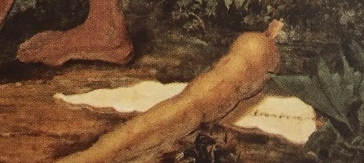
\includegraphics[width=60mm]{arcticles/02-farinha-e-carne-no-s/02-tupinamba-detalhe.jpg}};
\end{tikzpicture}


\vfill


\begin{tikzpicture}
    \node[inner sep=0pt] (plants) at (0, 0)
        {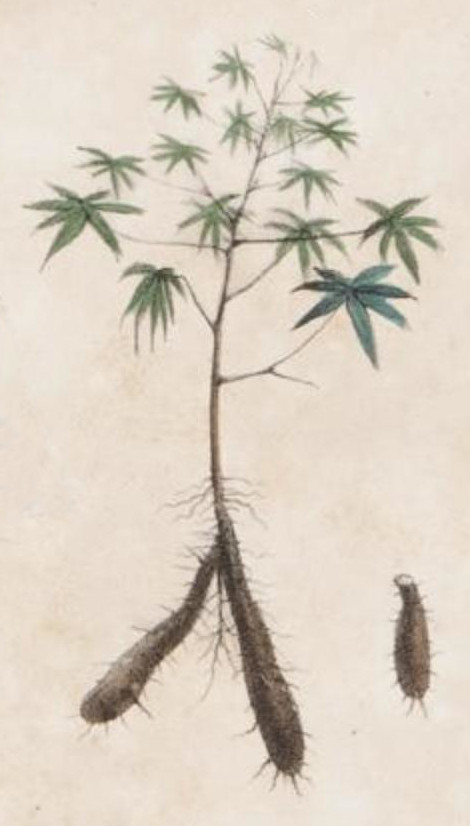
\includegraphics[width=50mm]{arcticles/02-farinha-e-carne-no-s/04-plantes-nutritives.jpg}};
    \node[inner sep=0pt, anchor=north west, text width=50mm, align=left]
    (subtitleone) at ([yshift=-5mm]plants.south west)
        {\small \textsf{Detalhe de \textit{Plantes Nutritivies} de Jean-Baptiste Debret. Litografia em cores, 51,4x33,4 cm. 1835.}};

    \node[inner sep=0pt, anchor=north west] (study) at ([xshift=21mm]plants.north east)
        {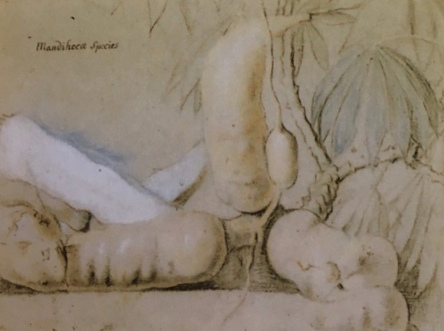
\includegraphics[width=45.4mm]{arcticles/02-farinha-e-carne-no-s/03-estudo-preparatorio-mandioca.jpg}};
    \node[inner sep=0pt, anchor=south west] (deadnature) at ([xshift=21mm]plants.south east)
        {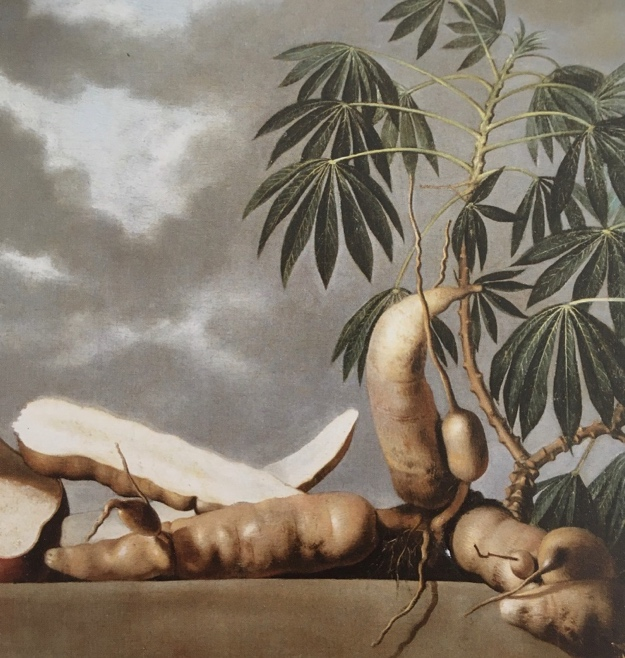
\includegraphics[width=45.4mm]{arcticles/02-farinha-e-carne-no-s/05-natureza-morta-mandioca.jpg}};
    \node[inner sep=0pt, anchor=north west, text width=47mm] (subtitletwo) at ([yshift=-5mm]deadnature.south west)
        {\small \textsf{\textit{Estudo preparatório} e \textit{Na\-tu\-re\-za-morta com man\-di\-o\-ca} de Albert Eckhout. Óleo sobre tela, 93x90 cm. 1640.}};
\end{tikzpicture}

\end{center}

\clearpage

\hspace*{-10mm}
\begin{tikzpicture}[every node/.style={inner sep=0,outer sep=0}]
    \node[] (engenho) at (0, 0)
        {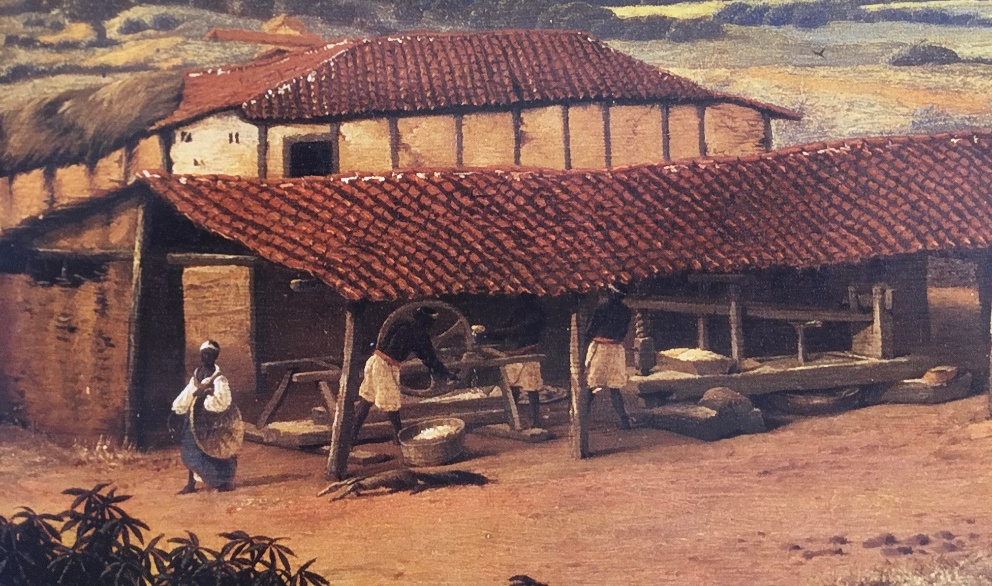
\includegraphics[width=97mm]{arcticles/02-farinha-e-carne-no-s/06-engenho-mandioca.jpg}};
    \node[anchor=east, text width=34mm, align=right] (caption) at ([xshift=-7mm]engenho.west)
        {\small \textsf{Detalhe de \textit{Engenho de mandioca} de Frans Post. Óleo sobre tela, 47x68 cm. 1651. Coleção particular, Inglaterra.}};
\end{tikzpicture}

\vfill

\hspace*{-16mm}
\begin{tikzpicture}[every node/.style={inner sep=0,outer sep=0}]
    \node[] (preparacao) at (0, 0)
        {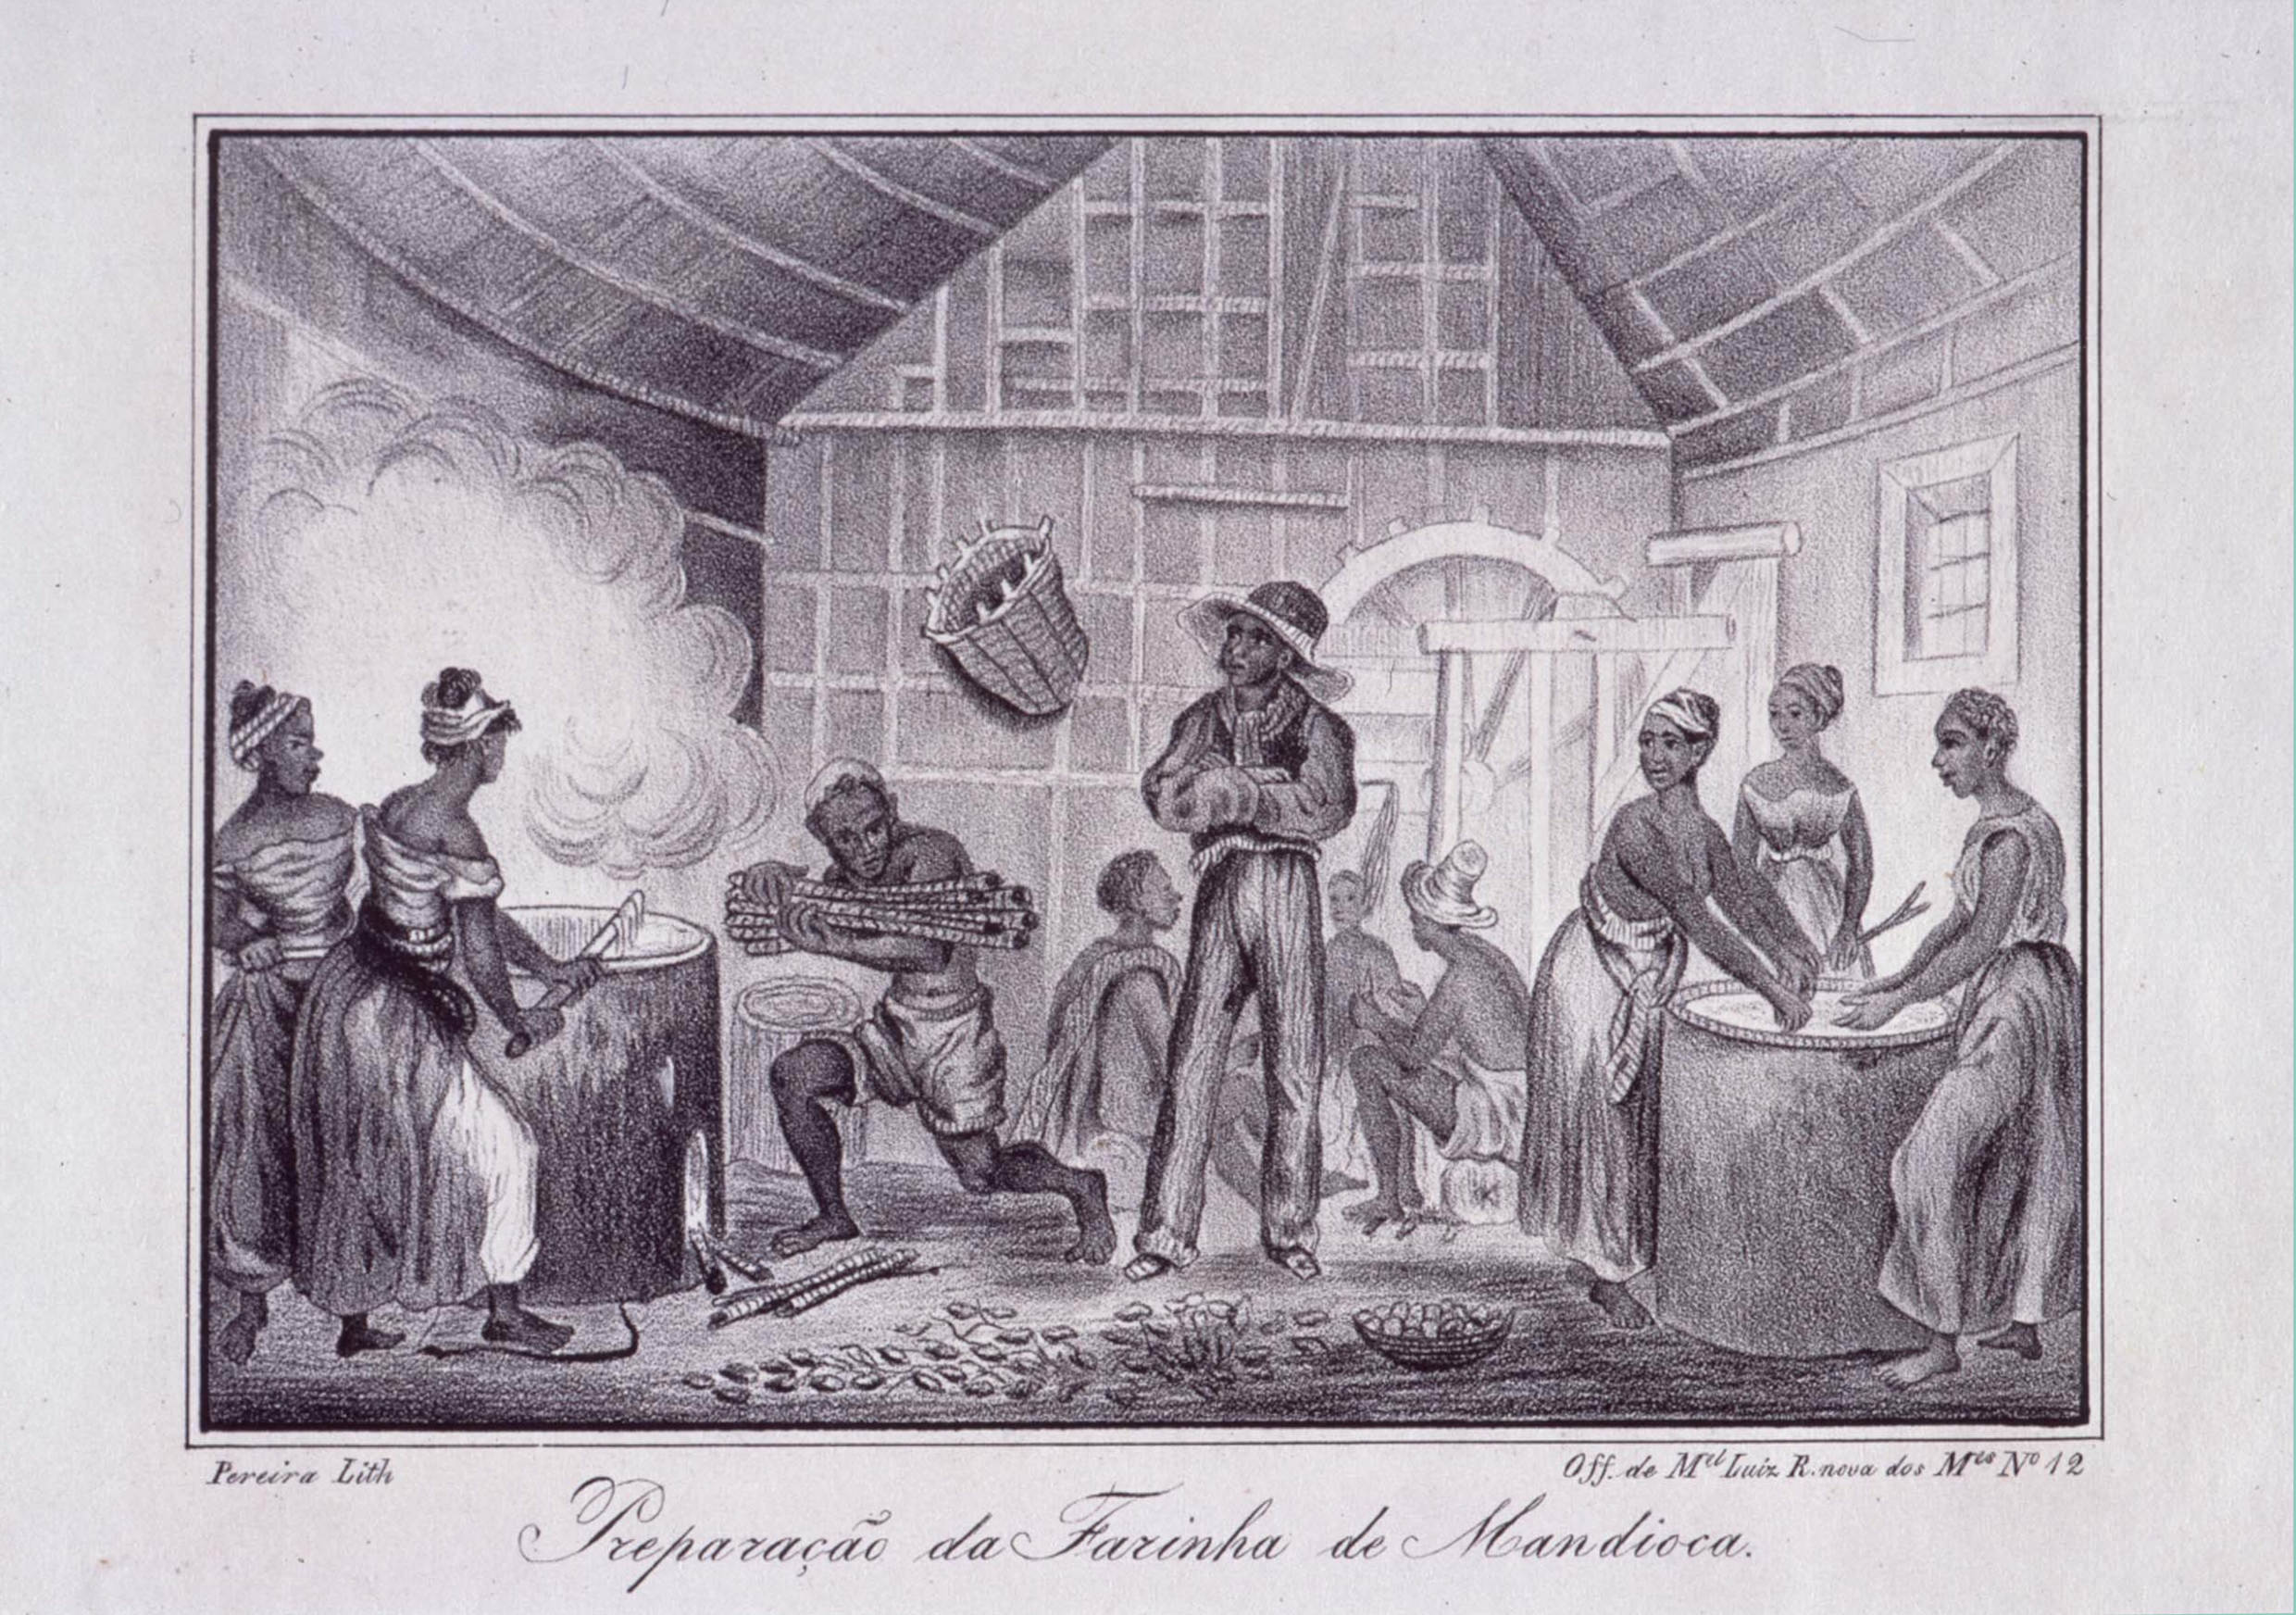
\includegraphics[width=103mm]{arcticles/02-farinha-e-carne-no-s/07-preparacao-farinha.jpg}};
    \node[anchor=west, text width=34mm] (caption) at ([xshift=7mm]preparacao.east)
        {\small \textsf{\textit{Preparação da farinha de mandioca} de Pereira. Litografia sobre papel, 13,9x18,5 cm. Século XIX. Arquivo Histórico Ultramarino.}};
\end{tikzpicture}

\vfill

\hspace*{-9mm}
\begin{tikzpicture}[every node/.style={inner sep=0,outer sep=0}]
    \node[] (eplucheuses) at (0, 0)
        {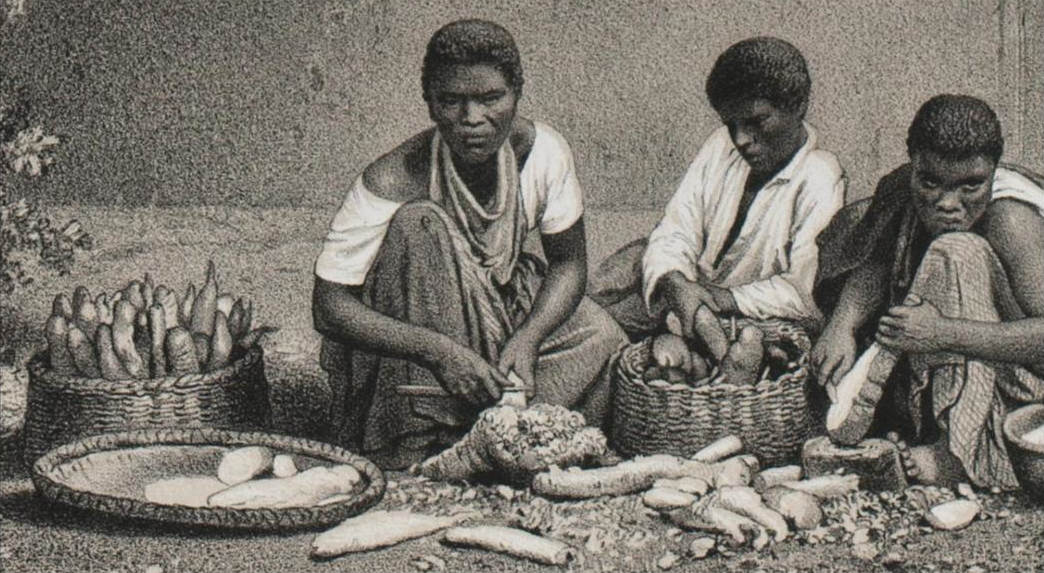
\includegraphics[width=96mm]{arcticles/02-farinha-e-carne-no-s/08-epluchiuses-mandioca.jpg}};
    \node[anchor=east, text width=34mm, align=right] (caption) at ([xshift=-7mm]eplucheuses.west)
        {\small \textsf{Detalhe de \textit{Éplucheuses de mandioca} de Victor Frond. Litografia sobre papel, 48x63,5 cm. 1861. Coleção particular, Inglaterra.}};
\end{tikzpicture}

\clearpage

\hspace*{-7.5mm}
\begin{tikzpicture}[every node/.style={inner sep=0pt,outer sep=0pt}]
    \node[] (tubinamba) at (0,0)
        {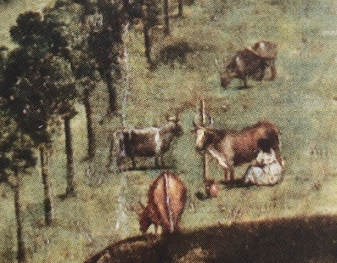
\includegraphics[width=73.5mm]{arcticles/02-farinha-e-carne-no-s/09-tupinamba-mulher-brazilian.jpg}};
    \node[anchor=west, text width=34mm] (caption) at ([xshift=7mm]tubinamba.east)
        {\small \textsf{Detalhe de \textit{Tupinambá/Mulher Brasilian} de Albert Eckhout. Óleo sobre tela, 274x163 cm. 1643.}};
\end{tikzpicture}

\vfill

\hspace*{5mm}
\begin{tikzpicture}[every node/.style={inner sep=0pt,outer sep=0pt}]
    \node[] (deux) at (0, 0)
        {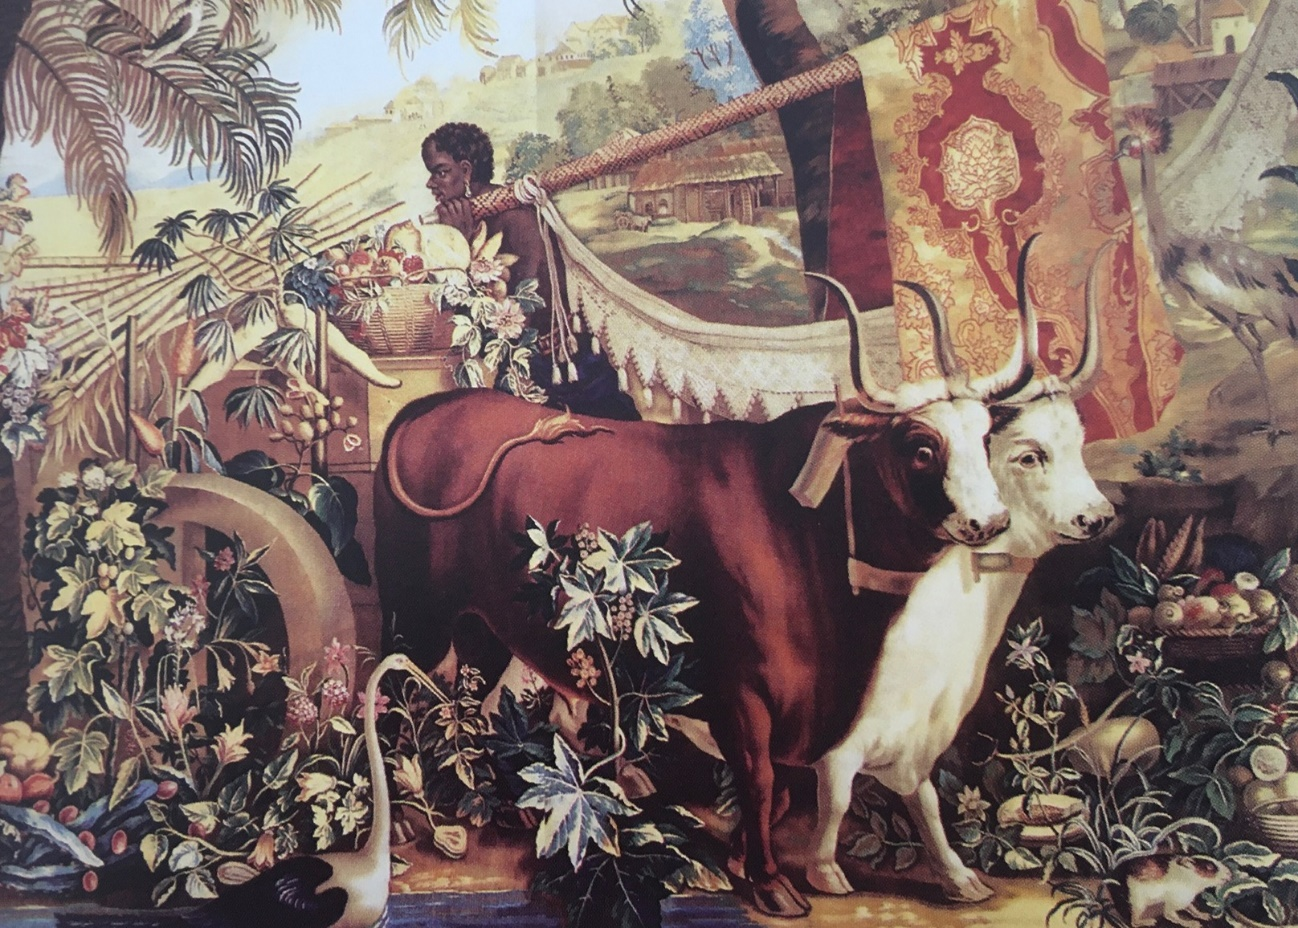
\includegraphics[width=82mm]{arcticles/02-farinha-e-carne-no-s/10-les-deux-taureaux.jpg}};
    \node[anchor=east, text width=34mm, align=right] (caption) at ([xshift=-7mm]deux.west)
        {\small \textsf{Detalhe de Tapeçaria a partir da obra de Albert Eckhout \textit{“Les deux taureaux”}. Lã e seda, 470x740 cm. Circa de 1690. Mobilier National de France.}};
\end{tikzpicture}

\vfill

\hspace*{-7.5mm}
\begin{tikzpicture}[every node/.style={inner sep=0pt,outer sep=0pt}]
    \node[] (transport) at (0, 0)
        {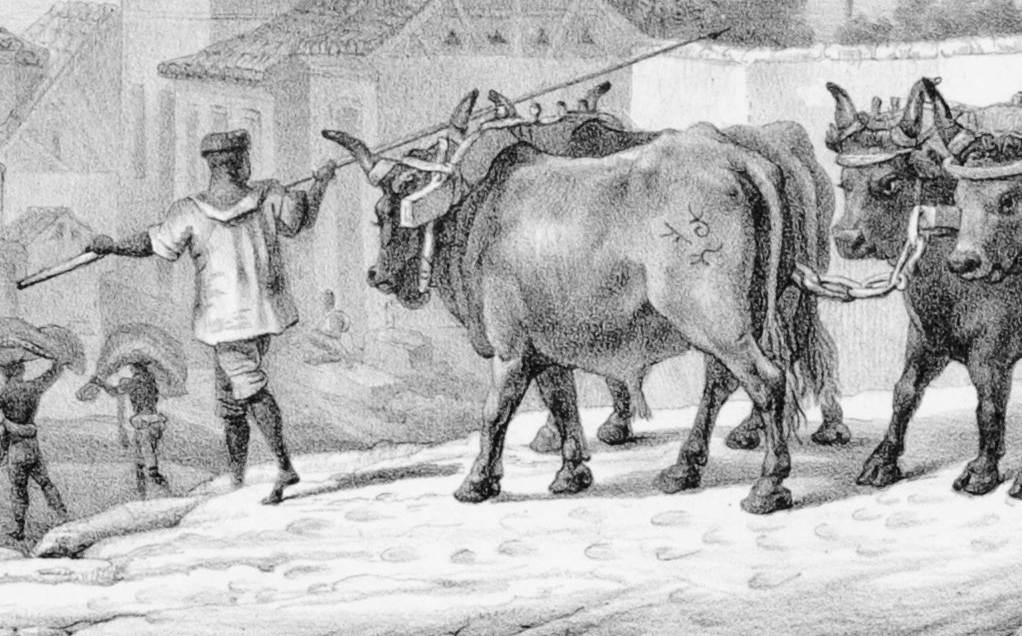
\includegraphics[width=85mm]{arcticles/02-farinha-e-carne-no-s/11-transport-des-viandes.jpg}};
    \node[anchor=west, text width=34mm] (caption) at ([xshift=7mm]transport.east)
        {\small \textsf{Detalhe de \textit{Transport de viande de boucherie} com marcas de propriedade no gado, de Jean-Baptiste Debret. Litografia em pb, 24,5x25,0 cm. 1835.}};
\end{tikzpicture}

\clearpage

\begin{vplace}
    \centering
    \begin{tikzpicture}
        \node[] (tratado) at (0, 0)
            {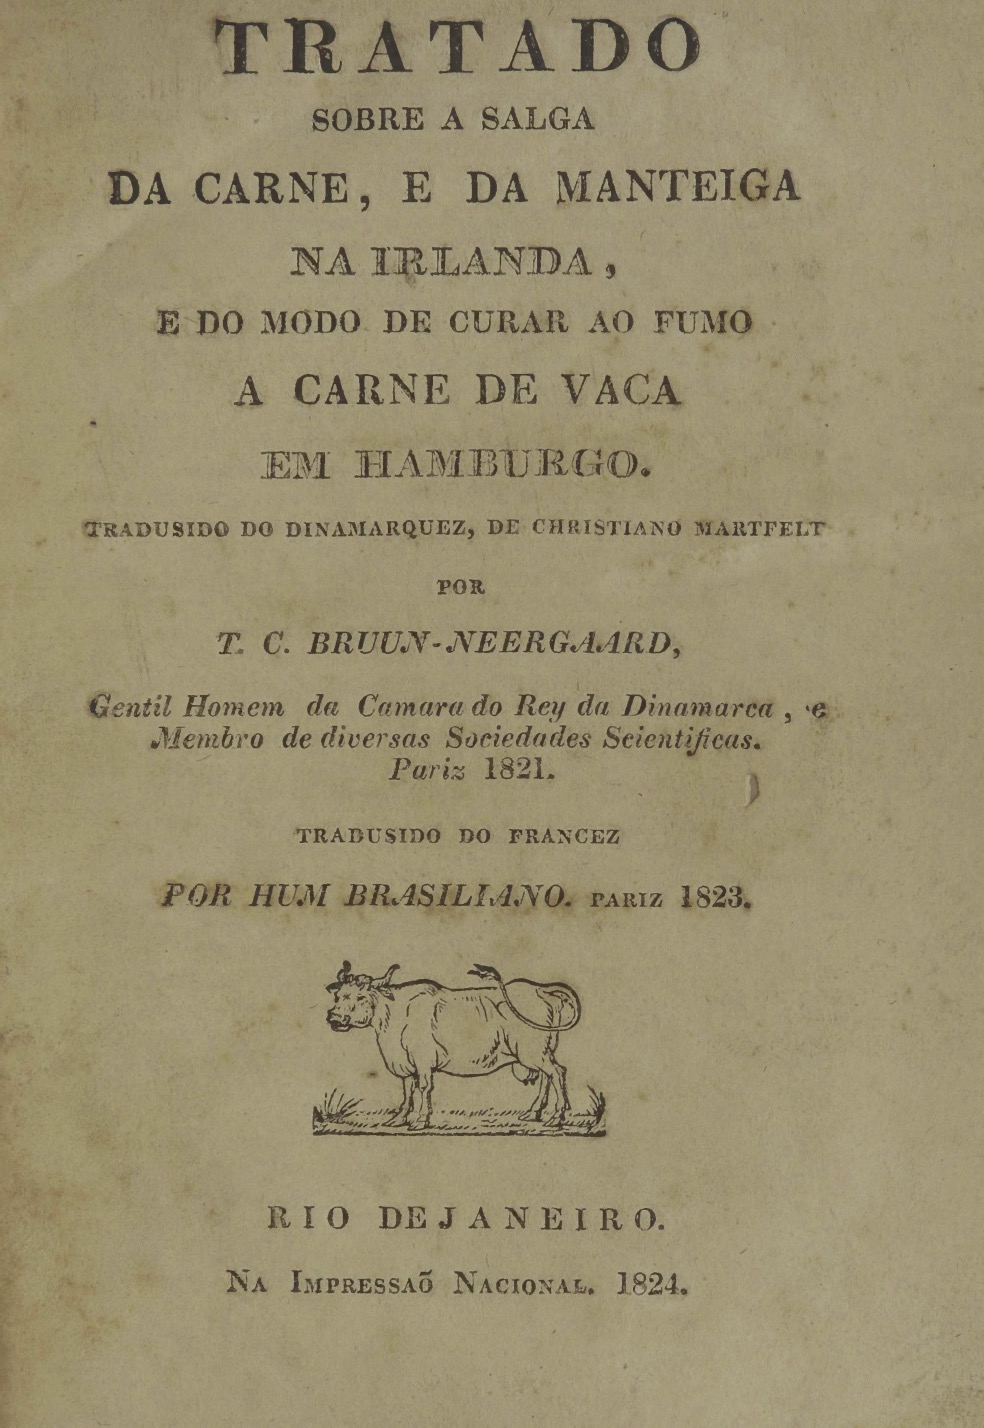
\includegraphics[width=93mm]{arcticles/02-farinha-e-carne-no-s/12-tratado-sobre-salga.jpg}};
        \node[anchor=north west, text width=93mm] (caption) at ([yshift=-5mm]tratado.south west)
            {\small \textsf{Capa do \textit{Tratado sobre a salga da carne\dots} de Christian Martfelt, traduzido do francês por um brasileiro e impresso no Rio de Janeiro em 1824.}};
    \end{tikzpicture}
\end{vplace}

\clearpage

\begin{vplace}
    \centering

    \begin{tikzpicture}[every node/.style={inner sep=0pt,outer sep=0pt}]
        \node[] (cozinheiro) at (0, 0)
            {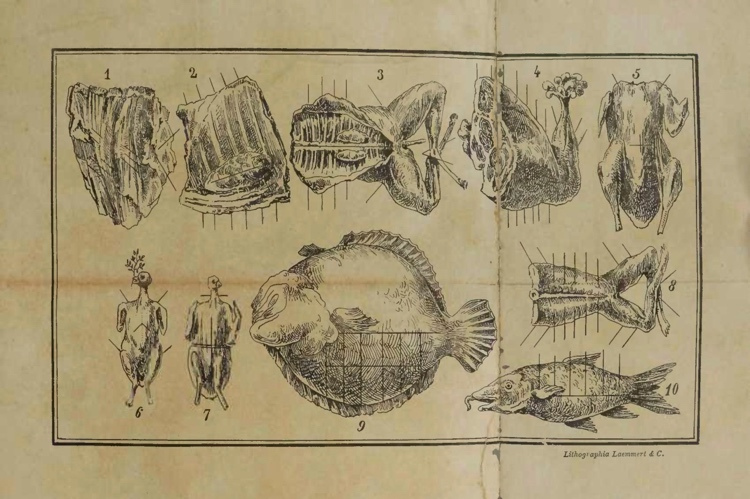
\includegraphics[width=72mm]{arcticles/02-farinha-e-carne-no-s/13-cozinheiro-imperial.jpg}};
        \node[anchor=south west] (detail) at ([xshift=7mm]cozinheiro.south east)
            {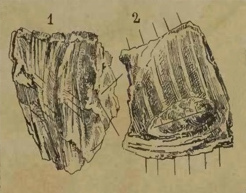
\includegraphics[width=43mm]{arcticles/02-farinha-e-carne-no-s/14-cozinheiro-imperial-detalhe.jpg}};
        \node[anchor=north west, text width=122mm] (caption) at ([yshift=-5mm]cozinheiro.south west)
            {\small \textsf{Detalhe do apenso da 10ª edição da obra \textit{Cozinheiro Imperial} (1ª ed. 1840) de 1887 mostrando os cortes de carne bovina de R. C. M e impresso no Rio de Janeiro em 1887.}};
    \end{tikzpicture}

    \vspace*{15mm}

    \begin{tikzpicture}[every node/.style={inner sep=0pt,outer sep=0pt}]
        \node[] (boutique) at (0,0)
            {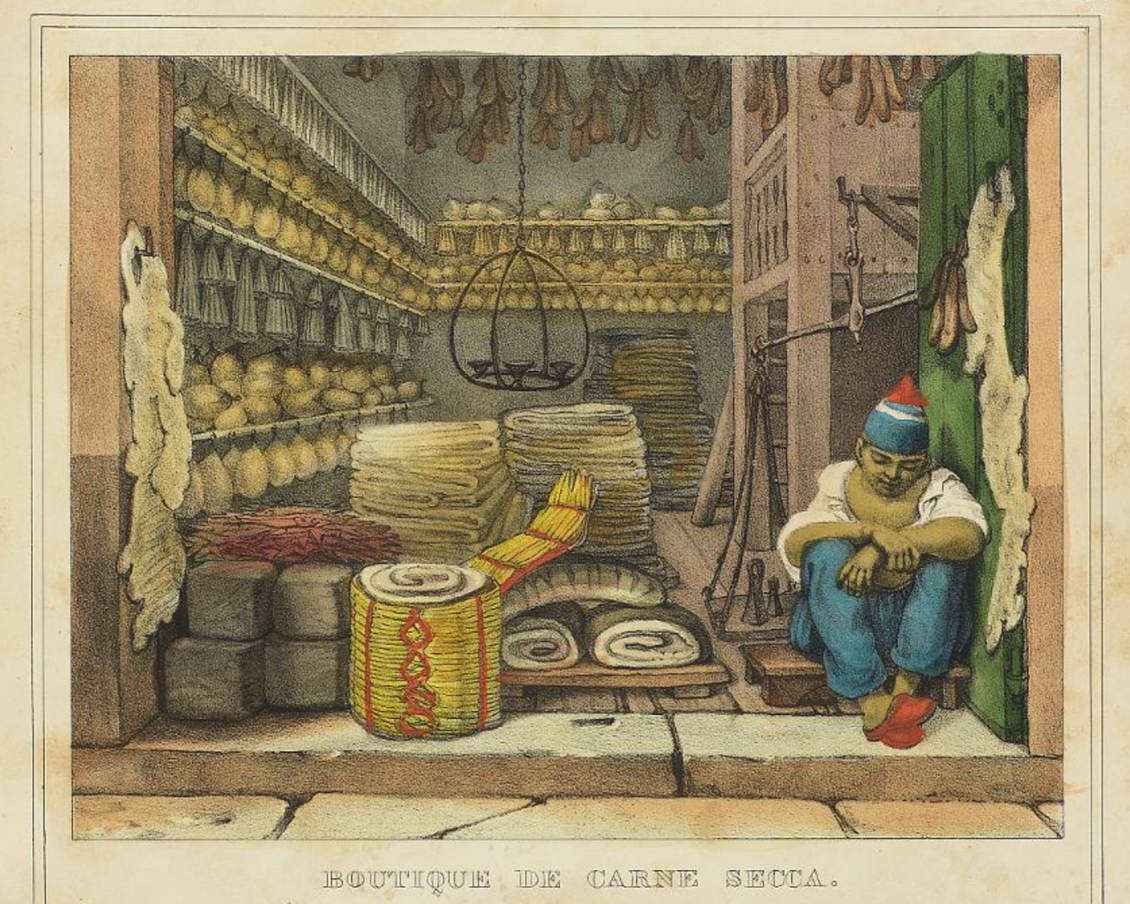
\includegraphics[width=96mm]{arcticles/02-farinha-e-carne-no-s/15-boutique-de-carne-secca.jpg}};
        \node[anchor=north, text width=82mm] (caption) at ([yshift=-5mm]boutique.south)
            {\small \textsf{\textit{Boutique de carne secca} de Jean-Baptiste Debret. Litografia em cores, 25,8x19,8 cm. 1835.}};
    \end{tikzpicture}

\end{vplace}

\clearpage

\begin{vplace}
    \centering

    \begin{tikzpicture}[every node/.style={inner sep=0pt,outer sep=0pt}]
        \node[] (a) at (0,0)
            {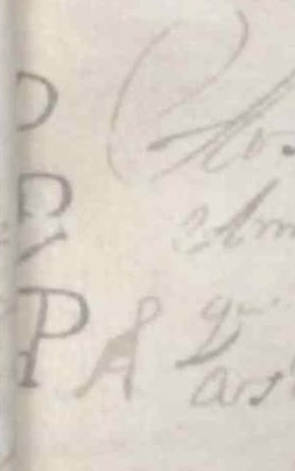
\includegraphics[width=31mm]{arcticles/02-farinha-e-carne-no-s/16-ferro-de-gado.jpg}};
        \node[anchor=south west] (b) at ([xshift=6mm]a.south east)
            {
\includegraphics[width=21mm]{arcticles/02-farinha-e-carne-no-s/17-ferro-de-gado-2.jpg}};
        \node[anchor=south west] (c) at ([xshift=6mm]b.south east)
            {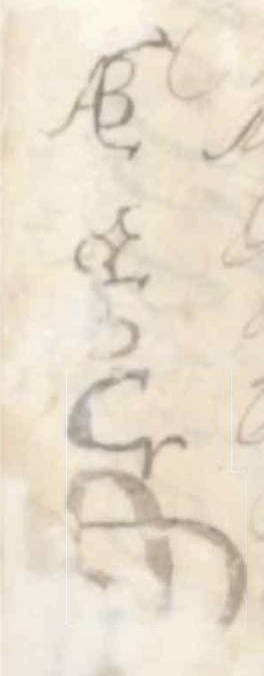
\includegraphics[width=27mm]{arcticles/02-farinha-e-carne-no-s/18-ferro-de-gado-3.jpg}};
        \node[anchor=south west] (d) at ([xshift=6mm]c.south east)
            {
\includegraphics[width=24.5mm]{arcticles/02-farinha-e-carne-no-s/19-ferro-de-gado-4.jpg}};
        
        \node[anchor=north west, text width=121.5mm] (caption) at ([yshift=-5mm]a.south west)
            {\small \textsf{\textit{Diversos registros de ferro do gado da Capitania do Rio Grande do Norte realizados na Câmara de Natal entre 1673 a 1690} constante no Livro de Registros de Cartas e Provisões da Câmara de Natal de 1673 a 1690.}};
    \end{tikzpicture}

    \vspace*{15mm}

    \begin{tikzpicture}[every node/.style={inner sep=0pt,outer sep=0pt}]
        \node[] (ferrosargento) at (0, 0)
            {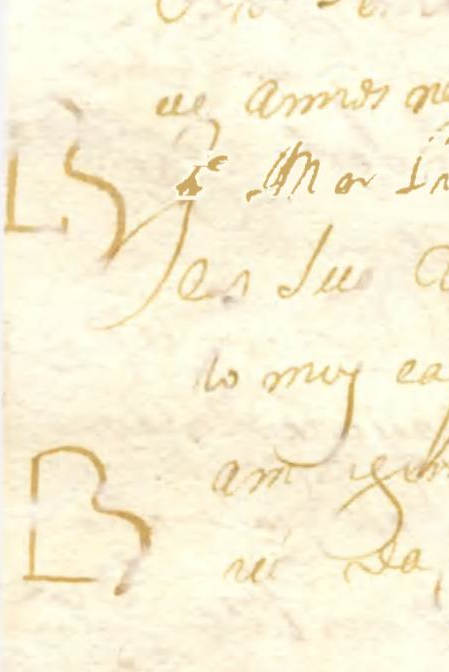
\includegraphics[width=46mm]{arcticles/02-farinha-e-carne-no-s/20-ferro-de-gado-sgto-mor-leo.jpg}};
        \node[anchor=west, text width=34mm] (caption) at ([xshift=7mm]ferrosargento.east)
            {\small \textsf{\textit{Registro de ferro do gado do Sargento-mor Leonardo Bezerra Cavalcante na Câmara de Natal em 6 de agosto de 1699} constante no Livro de Registros de Cartas e Provisões da Câmara de Natal de 1691 a 1702, p. 92v.}};
    \end{tikzpicture}
\end{vplace}

\clearpage

\begin{vplace}

    \hspace*{-7.5mm}
    \begin{tikzpicture}[every node/.style={inner sep=0pt,outer sep=0pt}]
        \node[] (desenhos) at (0, 0)
            {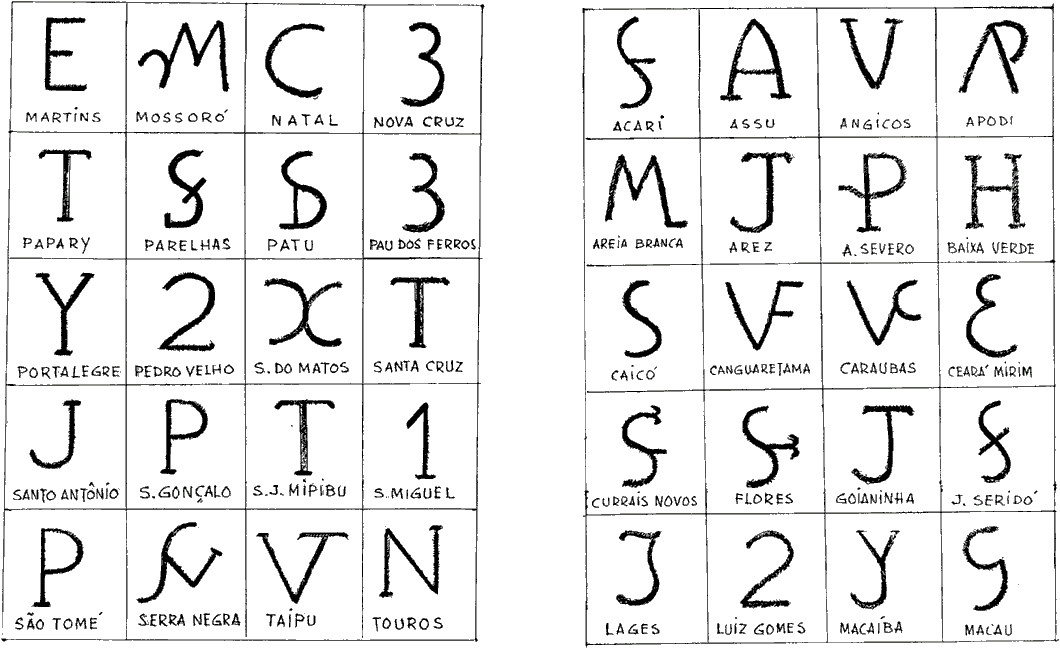
\includegraphics[width=136mm]{arcticles/02-farinha-e-carne-no-s/22-desenhos-marcas-de-ferro-2.png}};
        \node[anchor=north] at ([yshift=-6mm, xshift=2mm]desenhos.south)
            {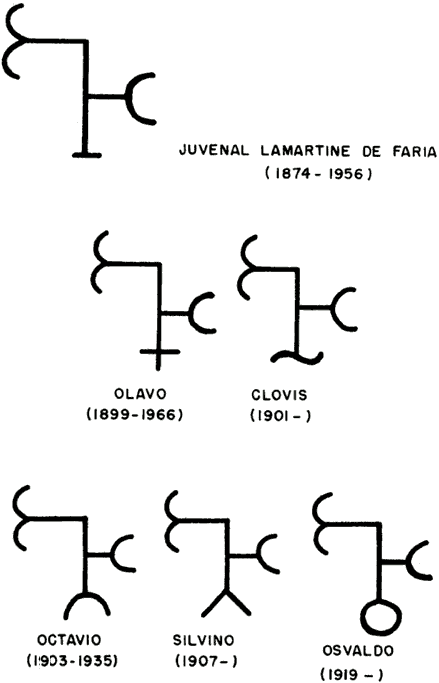
\includegraphics[width=56mm]{arcticles/02-farinha-e-carne-no-s/21-desenhos-marcas-de-ferro.png}};
        \node[anchor=south, text width=\textwidth] (caption) at ([yshift=5mm]desenhos.north)
            {\small \textsf{\textit{Desenhos utilizados nas marcas de ferro para gado do Rio Grande do Norte, séc. XIX--XX} por Oswaldo Lamartine de Faria em sua obra ``Ferro de Ribeiras do Rio Grande do Norte'' de 1984.}};
    \end{tikzpicture}
\end{vplace}

\end{refsection}
